\chapter{Resutls and Evaluation}

\begin{figure}
    \centering
    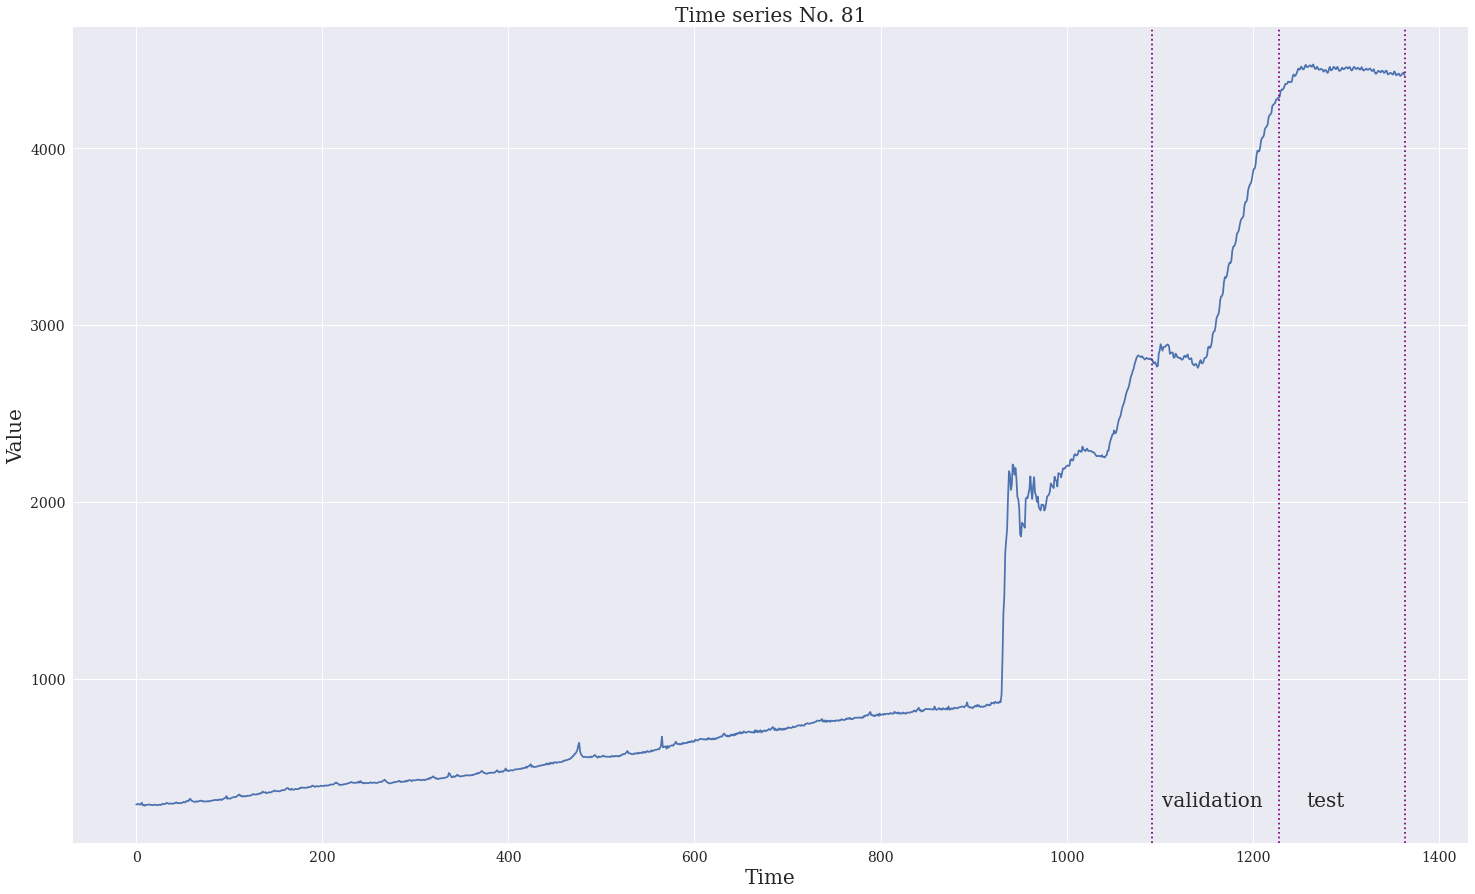
\includegraphics[width=15cm]{ts}
    \caption{ts}\label{fig: ts}
\end{figure}

\begin{figure}
    \centering
    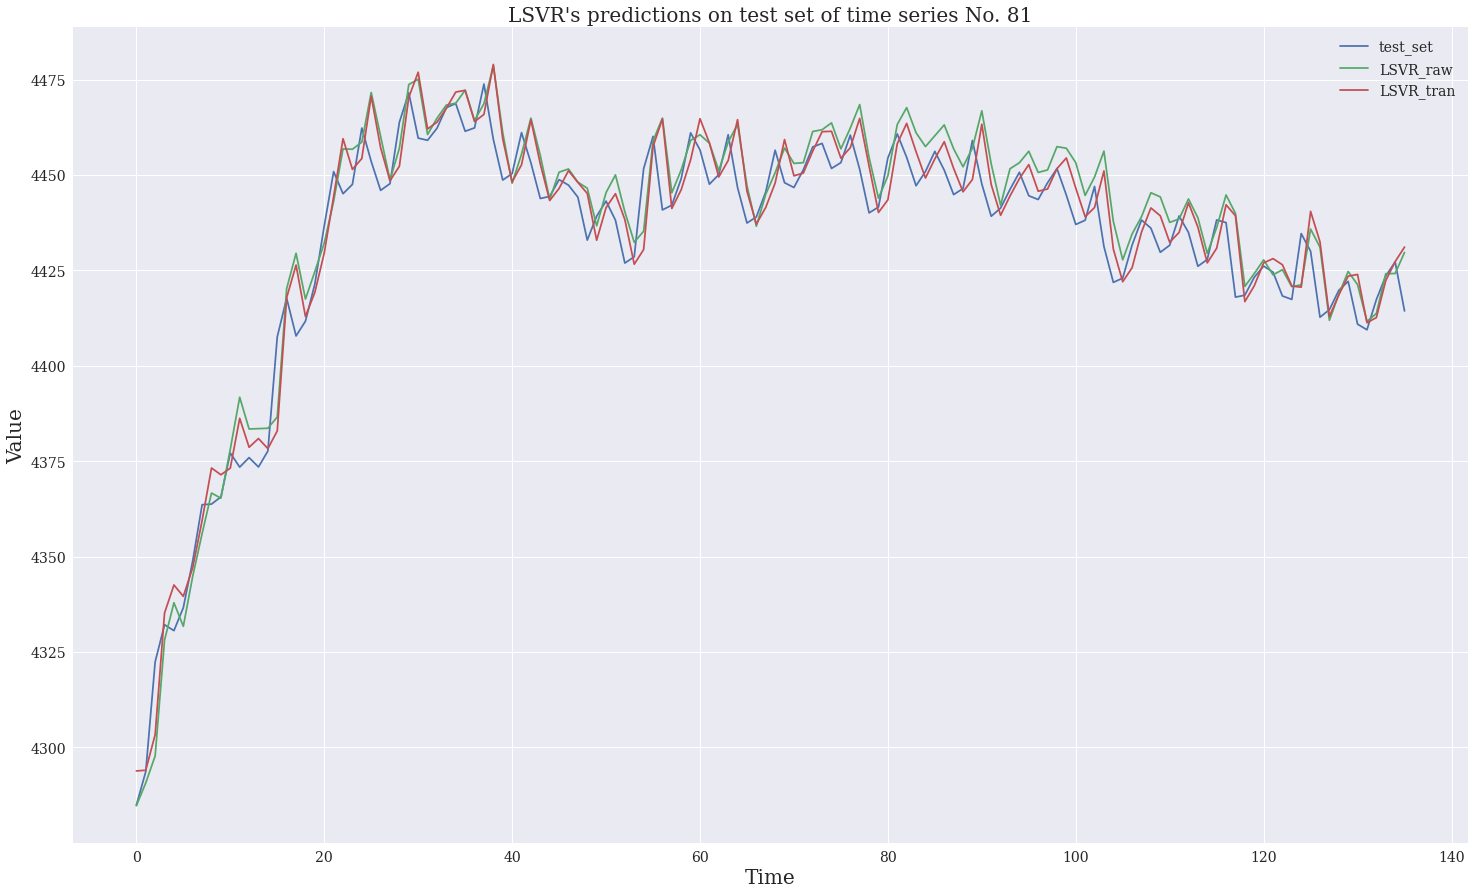
\includegraphics[width=15cm]{predict}
    \caption{predict}\label{fig: predict}
\end{figure}

\begin{figure}
    \centering
    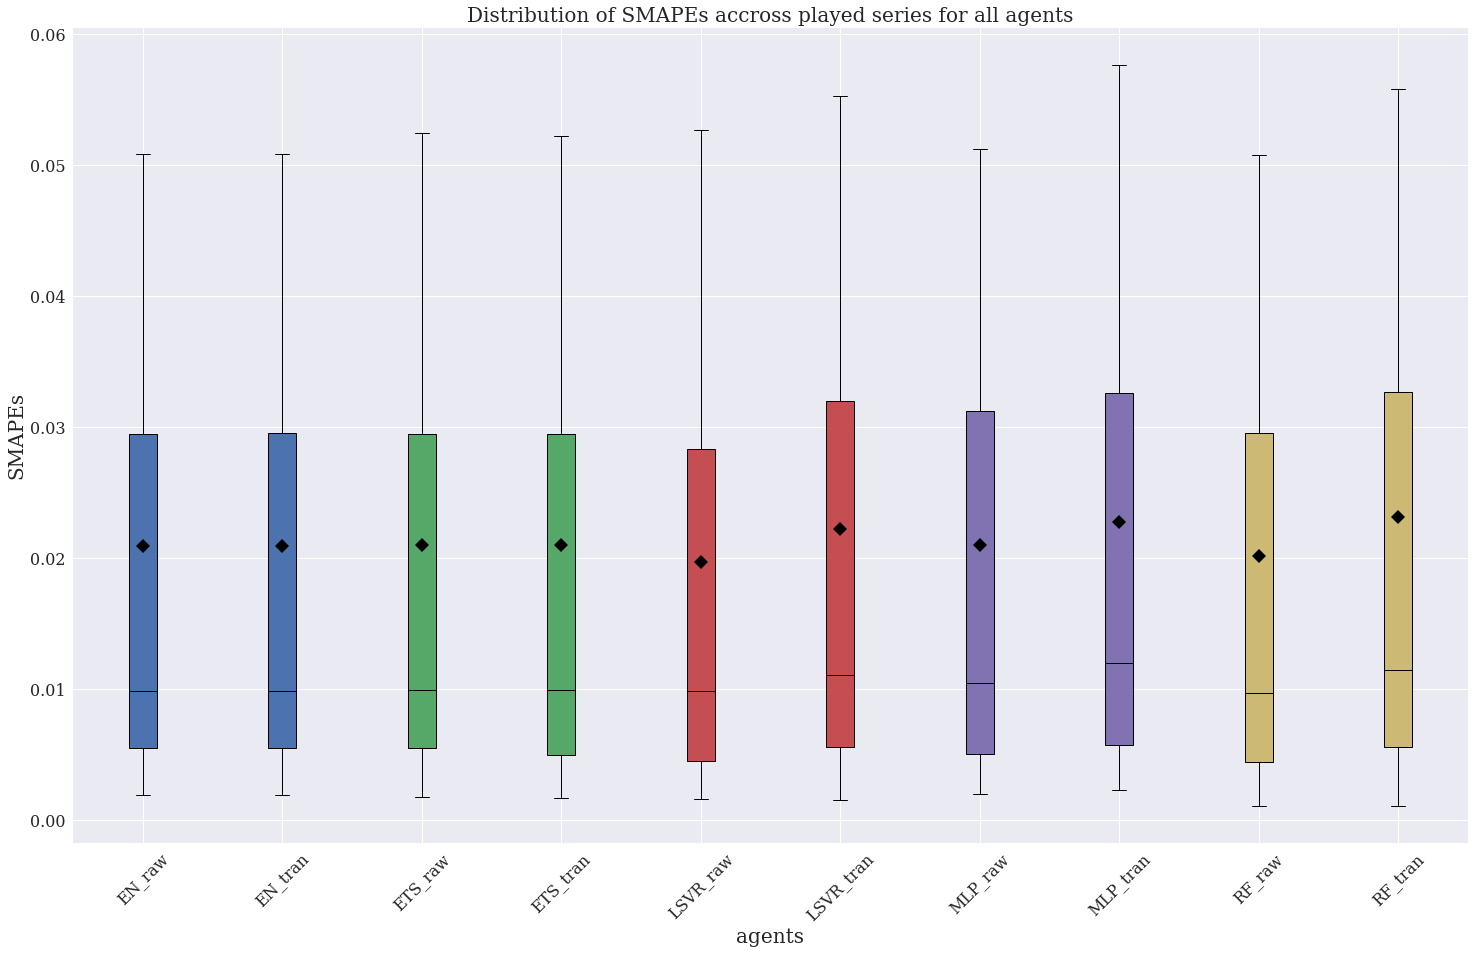
\includegraphics[width=15cm]{box}
    \caption{box}\label{fig: box}
\end{figure}

\begin{figure}
    \centering
    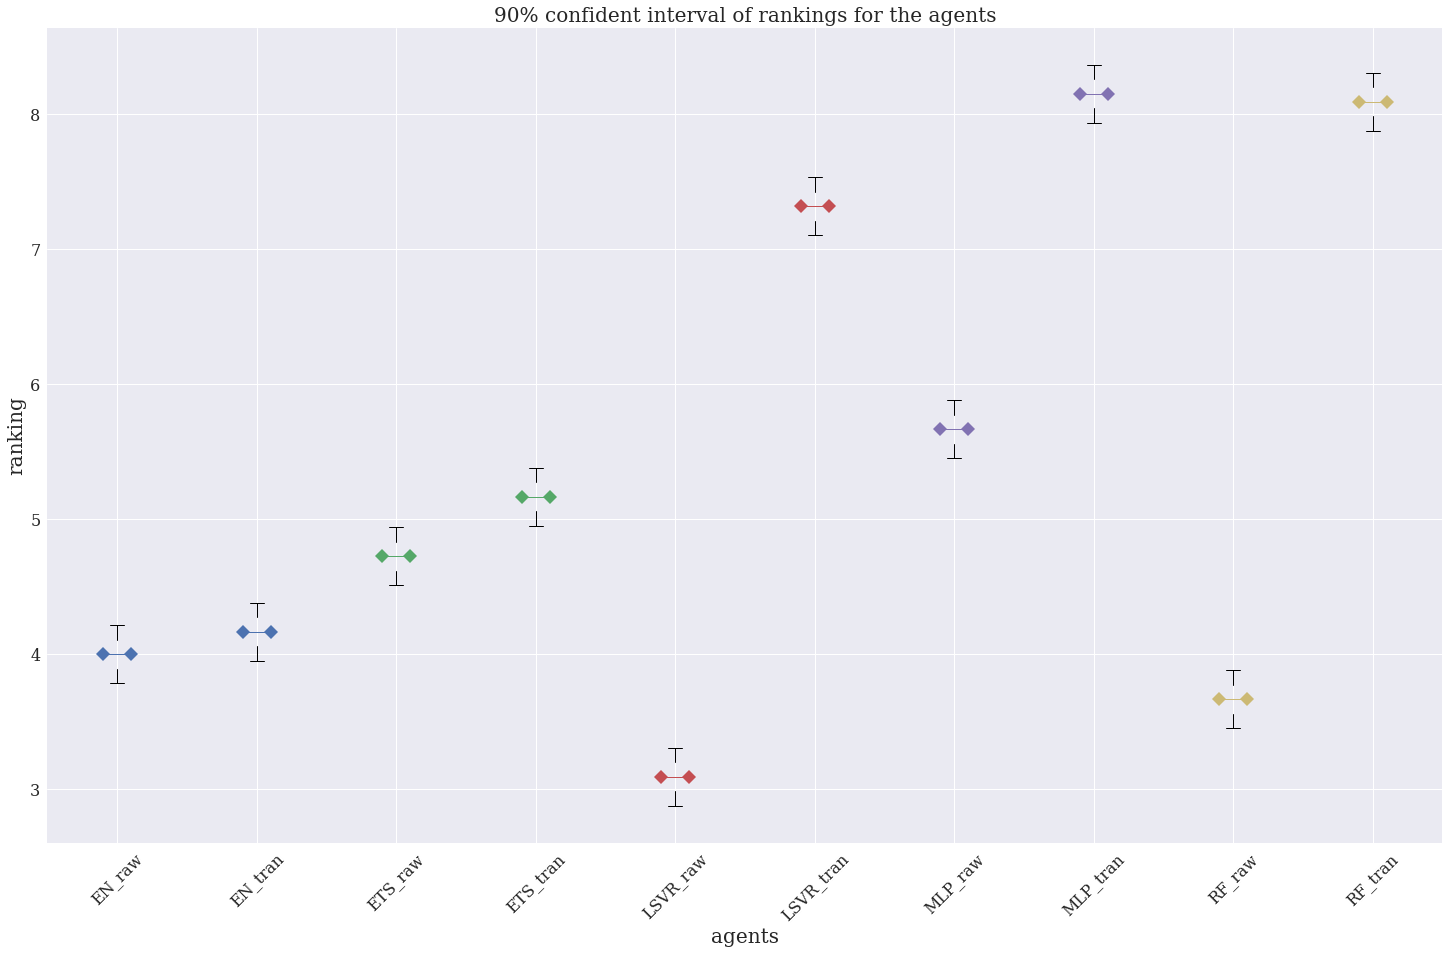
\includegraphics[width=15cm]{rank}
    \caption{rank}\label{fig: rank}
\end{figure}


\begin{center}
    \begin{table}
        \resizebox{\columnwidth}{!}{\begin{tabular}{|l|llllll|}
            \hline
            {} & mean SMAPE & std. SMAPE & mean rank & std. rank & 90\% rank interval & frac best \\
            \hline\hline
            EN\_raw    &    0.02091 &   0.024271 &          4.0 &        1.954 &            (3.753, 4.247) &     0.121 \\
            EN\_tran   &   0.020935 &   0.024349 &        4.167 &        1.919 &             (3.92, 4.414) &     0.106 \\
            \hline
            ETS\_raw   &   0.020979 &   0.024556 &        4.727 &        2.042 &             (4.48, 4.974) &     0.061 \\
            ETS\_tran  &   0.021029 &    0.02474 &        5.167 &        2.086 &             (4.92, 5.414) &      0.03 \\
            \hline
            LSVR\_raw  &   0.019724 &   0.022382 &        3.091 &        2.227 &            (2.844, 3.338) &     0.348 \\
            LSVR\_tran &   0.022205 &   0.024924 &        7.318 &         2.14 &            (7.071, 7.565) &     0.015 \\
            \hline
            MLP\_raw   &   0.021029 &   0.023338 &        5.667 &        2.749 &             (5.42, 5.914) &      0.03 \\
            MLP\_tran  &   0.022734 &   0.024506 &        8.152 &        2.251 &            (7.905, 8.399) &       0.0 \\
            \hline
            RF\_raw    &   0.020129 &   0.022872 &        3.667 &        2.809 &             (3.42, 3.914) &     0.348 \\
            RF\_tran   &    0.02314 &   0.026118 &        8.091 &        2.598 &            (7.844, 8.338) &     0.045 \\
            \hline
        \end{tabular}}
        \caption{Test statistics on weekly financial time series}
        {\raggedright The dataset consists of $71$ time series. Average length of the time series is $1260.
        70$. \par}
        \label{tbl: weekly finance stats}
    \end{table}
\end{center}

